%
% Chapter 2
%

\chapter{THEORY}
\section{The Standard Model}
The Standard Model (SM) of particle physics is one of the most elegant descriptions of nature available. It explains three of four fundamental forces via gauge symmetries, while characterizing unknown matter into
separate generations of particles called quarks and leptons. Since its inception in the early 1960s, the SM has predicted the existence of every fundamental particle that has been discovered to-date.
The SM distills the real-world observables matter and energy into discrete elementary particles and their kinematics. The SM is the theory on which all of the following research is based, and also the hypothesis being tested in this analysis.

\subsection{Particle Content}
The particles in the SM are first characterized by their intrinisic angular momentum, more commonly referred to as spin. Particles with half-integer spin, quantized in units of Planck's constant $\hbar$, are fermions, while particles with integer spin are bosons.
This distinction is important because the spin values govern behavior and interactions of collections of particles. 

The fermions in the SM are the most fundamental examples of matter in nature. Fermions behave and interact according to Fermi-Dirac statistics, and obey the Pauli exclusion principle. Fermions are further categorized, based on their primary interaction mechanism,
into quarks and leptons. There are six different flavors of quarks in the SM, the up and down, the charm and strange, and the top and bottom quarks are organized into three generations of doublets below.
\begin{equation}
\binom{u}{d} \;\;\; \binom{c}{s} \;\;\; \binom{t}{b}
\end{equation}
\noindent An increasing mass (from left to right) distinguishes each generation, while the upper and lower elements of each doublet are distinguished by an electric charge of +2/3 and -1/3 respectively in each generation. Quarks interact via the strong and
electroweak forces. Quarks also carry a color charge, which can assume one of three values (red, blue, green) as a result of the strong interaction described by Quantum Chromodynamics (QCD). The leptons in the SM can also be arranged into three increasingly
massive generations of doublets.
\begin{equation}
\binom{e^{-}}{\nu_{e}} \;\;\; \binom{\mu^{-}}{\nu_{\mu}} \;\;\; \binom{\tau^{-}}{\nu_{\tau}}
\end{equation}
\noindent The upper elements in each lepton doublet are the familiar electron, and the less familiar but much heavier, muon and tau. Due to their increased mass, the muon and tau have very short lifetimes which causes them decay rapidly
to lighter, more stable particles. The electron, muon, and tau all have the same electric charge of -1. The lower elements in each doublet are the lightweight and electrically neutral counterparts called neutrinos, which also come in three
flavors; the electron-neutrino, the muon-neutrino, and the tau-neutrino. Neutrinos interact primarily through the weak force. In an experimental context such as CMS, neutrinos are characterized by
how weakly they interact. They effectively don't interact at all for what concerns CMS. They interact so weakly that they are able to pass through all of planet earth without a single interaction.
This property makes it impossible to directly detect their presence at CMS. 

\begin{figure}[hbtp]
 \begin{center}
   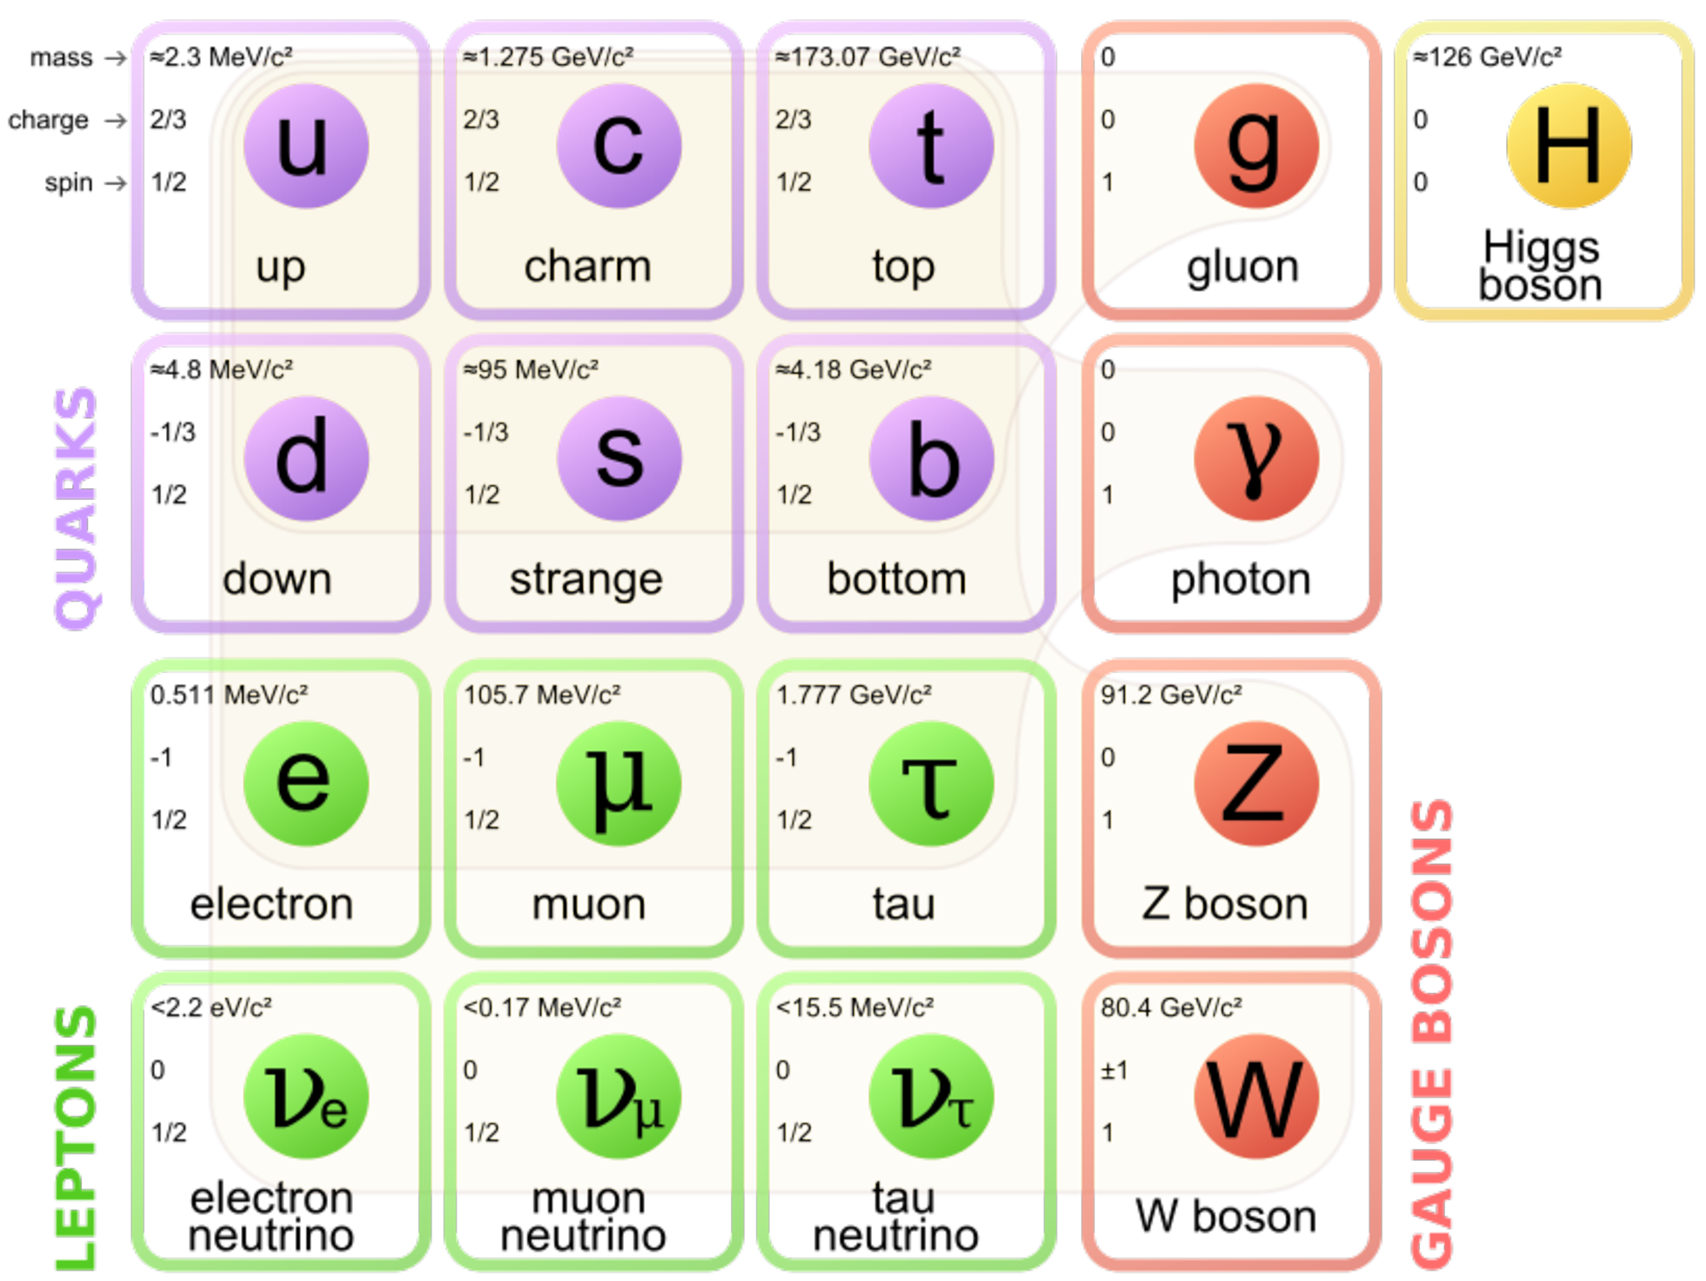
\includegraphics[width=0.8\textwidth]{ch2_figs/sm_particles_periodic_table.pdf}
   \caption{A sumamry of all elementary particles and their interactions in the Standard Model~\cite{sm_table}.}
   \label{fig:sm_periodic_table}
 \end{center}
\end{figure}

The bosons in the SM are also fundamental, but are not examples of matter. Bosons are characterized by their integer-quantized angular momentum and behave according to Bose-Einstein statistics. There are five elementary SM bosons, the four force-carrying gauge
bosons, and one scalar (spin-0) boson that was recently discovered in 2012, known as the Higgs boson. The four forces (strong, weak, electromagnetic, gravity) through which particles interact are all
carried by corresponding gauge bosons. The SM currently does not explain or incorporate gravity and as such there is no SM particle that carries its force. The hypothetical gauge boson believed to be responsible for gravity is the graviton,
and has yet to be discovered because likely exists in a mass range far beyond the reach of today's colliders like the LHC.
The strongest of the four forces, the appropriately-named strong force is carried by the gluon. Gluons are spin-0, electrically neutral, massless, and carry a color charge. Gluons mediate the strong force through which quarks interact. Due to the nature of
color charge and confinement, gluons keep the quarks inside protons and neutrons \emph{glued} together, confined inside the proton. Additionally, strong force also binds protons and neutrons together to form nuclei of atoms. Any particle carrying color-charge
is capable of strong interactions. 
The photon is the gauge boson that mediates the next strongest interaction, the electromagnetic force. The photon is massless, spin-1, electrically neutral, and travels at the speed of light. Aside from gravity, the electromagnetic force is the most familiar,
responsible for keeping electron orbitals bound to nuclei, forming atoms, and it is also responsible for the attractive and repulsive forces that bond atoms together into molecules. Any particle carrying electric charge is capable of interacting electromagnetically.
The weakest force explained by the SM, the appropriately named weak force is mediated by the massive W and Z gauge bosons. There are two types of weak interactions, charged and neutral.
There are two W bosons, W$^+$,W$^-$ which are identical except for their electric charges of +1 and -1 respectively. The spin-1 W boson has a mass of 80.4 GeV~\cite{pdg}, and mediates the weak charged interaction.
The electrically neutral, spin-1 Z boson has a mass of 91.2 GeV and mediates the weak neutral interaction~\cite{pdg}. The decay of unstable atoms, which is harnessed for nuclear power, is possible thanks to the weak interaction.
The final elementary SM boson is the Higgs. The Higgs is a massive spin-0, electrically neutral boson that interacts with both fermions and other bosons and has a mass of approximately 125 GeV~\cite{pdg}. While the Higgs doesn't mediate a force,
it does represent a field and the
mechanism by which elementary particles (matter) obtain masses. The Higgs boson and the origins of mass will be explained the coming sections. 

\begin{table}[hbtp]
\centering
\caption{Relative dimensionless strengths of the fundamental forces}
\begin{tabular}{lcc}
\hline
Force & Relative Strength \\
\hline
Gravity & $1$ \\
Weak &  $10^{25}$ \\
Electromagnetic & $10^{36}$ \\
Strong & $10^{38}$ \\
\hline
\end{tabular}
\label{tab:force_table}
\end{table}


\subsection{Fields and Symmetries}
The notion of symmetry is of central importance to the SM.
The SM describes three of the fundamental forces with gauge field theories.
A gauge theory is a field theory whose Lagrangian is invariant under a specific type
of transformation, called a gauge transformation. These transformations form a symmetry (group), because the Lagrangian is invariant under the transformation.
The word symmetry is used to describe these transformations because
the underlying dynamics of the theory are left unchanged or \emph{symmetric} with respect to the transformation.
Thanks to Noether's Theorem, these symmetries are critical to the SM because they describe and invoke the convservation laws that SM particles obey.
Each force within the SM corresponds to its own gauge field theory
and symmetry that describe it. In each gauge theory, the corresponding field or force-carrying gauge boson is represented by the generators of the symmetry group. 

Originally, the gauge theory that described the electromagnetic force, Quantum Electrodynamics (QED), was invariant under a $U(1)$ symmetry that described the photon as the
force-carrying gauge boson and the symmetry required electric charge to be conserved. QED was first developed by Sinitoro Tomononga, Julian Schwinger, and Richard Feynman.
This laid the foundation on which the rest of the SM was built and won them the Nobel Prize in 1965~\cite{NP65}. 

Not long after the development of QED, C.N. Yang and Robert Mills formalized the gauge field theory techniques that were further refined by Sheldon Glashow, Abdus Salam,
and Steven Weinberg in the 1960s to combine QED
with the description of the weak force, producing a unified electroweak theory that described electromagnetism and the weak force~\cite{NP79}.
%%continueing paragraph
With this unification came new quantum numbers and conservation laws associated with the electroweak force. Among them are the conserved quantities of isospin and hypercharge\footnote{Also commonly
referred to as weak isospin and weak hypercharge}. These conserved quantites are actually used to redefine the already-conserved and familiar quantity of electric charge

\begin{equation}
\label{eqn:hypercharge}
Q = T_{3} + \frac{Y_{W}}{2}
\end{equation}
 
\noindent where $Q$ is the familiar electric charge, $T_{3}$ is the third component of isospin and $Y_{W}$ is the hypercharge. With these newly introduced quantum numbers,
the notion of helicity or handedness is now very relevant
in describing the electroweak force. Helicty is defined as the orientation of a particle's spin vector to its linear momentum vector. Particles are said to be lefthanded  when their spin vector is antialigned with
their linear momentum vector ($T_{3}=\pm 1/2$), and righthanded ($T_{3}=0$) when the two vectors are aligned.  
This unified electroweak theory is a
$U_{Y}(1) \otimes SU_{L}(2)$ gauge theory, where Y represents the weak hypercharge, and L means that only left-handed fermions participate in the weak interaction. 
The corresponding gauge bosons are the massless photon, and the massive weak force-carriers the W and Z. The initial problem with the electroweak theory was that there was no
mechanism in place to describe massless force carriers other than the photon. The solution to this problem, and its implications for the Higgs boson are described in the
following section.

The remaining gauge theory necessary for the SM is QCD. The theoretical underpinnings of QCD were developed in 1965 by Moo-Young Han, Yoichiro Nambu, and Oscar Greenberg, after
significant work from Murray Gell-Mann and others describing the interactions of quarks~\cite{QCD}.  
Unlike the QED, QCD is a non-abelian gauge field theory. The consequence of this is that the force-carrying gauge boson
of QCD, the gluon, can interact with itself (and other gluons). This non-abelian gauge theory is denoted as $SU_{c}(3)$, with the conserved property of QCD being color charge.
Bare color-charged particles
cannot exist alone, rather they are confined to color-neutral states. Everyday examples of this include baryons (which include protons and neutrons) where each constituent quark
carries a unique color charge. At very short distances and very high energies however, it is possible to observe an approximately unconfined quark, however the strong confining
forces increases with increasing distance between color charges until it becomes energetically favorable to generate a new color-neutral quark-antiquark pair from the vacuum.
This process, known as fragmentation, has very important consequences in the context of experimental physics at CMS, as the hard collisions often produce bare quarks.
The experimental techniques used to detect and reconstruct these bare quarks and their fragmentation components is described in the following chapters. 

Combining electroweak theory with QCD, we have the SM, an $U_{Y}(1) \otimes SU_{L}(2) \otimes SU_{c}(3)$ gauge field theory that describes all interactions and particles in
Figure~\ref{fig:sm_periodic_table}. The remaining unexplained portions of electroweak theory, and their implications on particle masses and the Higgs boson is explained next.   

\subsection{Electroweak Symmetry Breaking}

In electroweak $U_{Y}(1) \otimes SU_{L}(2)$ gauge theory, gauge invariance requires all of the force-carrying gauge bosons to be massless.
For everything to make sense, the weak force-carrying W and Z gauge bosons would need to be massless, just like the photon. 
However the W and Z are massive, as are the fermions in the theory. Enter electroweak spontaneous symmetry breaking (EWSB). Thanks to the identification of EWSB, in 1964 
three groups almost simultaneously explained the origins of particle masses using EWSB and gauge invariance in what became known as the 1964 PRL symmetry breaking papers
~\cite{1964_prl_englert}~\cite{1964_prl_higgs}~\cite{1964_prl_guralnik}.
The explanation by which particles aquire masses is the Higgs Mechanism. For the particles in electroweak theory to have mass, they must be coupled to a field.
Adding the Higgs field to the electroweak Lagrangian and imposing gauge invariance gives masses to the W and Z gauge bosons as well as the fermions, but it does not interact
or give mass to the photon. Giving mass to the W and Z but not the photon spontaneously breaks the $U_{Y}(1) \otimes SU_{L}(2)$ symmetry.
Adding the Higgs field to the electroweak Lagrangian must be done in such a way as to minimize the new potential. The addition of the Higgs field means that new potential
is minimized at a non-zero value. This non-zero value is referred to as the vacuum expectation value (V.E.V.) and is the ground state of the SM.
The fields in the SM are considered fluctuations around the V.E.V. The addition of the Higgs field and minimization of the potential to the resulting ground state
is said to spontaneously break the symmetry because no external impetus for it exists. A famous and more intuitive example of spontaneous symmetry breaking can be illustrated
by imagining a plastic ruler and holding it vertically between your hands and then compressing your hands so that the center of the ruler bows to the right or the left and
spontaneously breaks the right left symmetry of the ruler-hand system~\cite{robinson}. 
This Higgs field, similar to the gauge fields, is represented by a particle the Higgs boson.
For the field to give all electroweak particles mass, it interacts with bosons and fermions.
The interaction of the Higgs boson (or any boson) with fermions is known as the Yukawa interaction or coupling. The strength of the Yukawa coupling
of the Higgs boson with fermions is the primary focus of this dissertation. Finally, 

\subsection{The Higgs Boson}

The particle manifestation of the Higgs field is the Higgs boson. After the Higgs mechanism was first introduced in 1964 to explain the origins of particle mass,
the race was on to experimentally confirm the massive gauge bosons predicted by the unified electroweak gauge theory including the Higgs mechanism ~\cite{higgs}.
The W and Z were discovered and their masses confirmed in 1983 by the UA1 and UA2 experiments at the Super Proton Synchrotron (SPS) at CERN ~\cite{WandZdiscoveries}.

The missing piece of the puzzle was the Higgs boson and the search was on. The Large Electron Positron Collider (LEP) at CERN was the next place to look for the Higgs.
Beginning in 1989 experiments at LEP searched for the Higgs at center-of-mass energies ranging from 45 GeV early on, ending at over 200 GeV in 2000. Meanwhile, Higgs
searches were also being conducted at the Tevatron collider at Fermilab. The Tevatron reached higher collision energies than LEP, with its second run lasting from 2001
to 2011, colliding protons and anti-protons at a center-of-mass energy 10x greater than that of LEP, reaching nearly 2 TeV. The next collider, the Large Hadron Collider
(LHC) at CERN came online in 2008. The search for the Higgs came to an end when the ATLAS and CMS experiments announced the discovery of the Higgs in 2012 at the LHC. 

Almost 48 years after being theorized, the Higgs discovery proved the existence
of the Higgs field, and validated the Higgs mechanism as well as the SM. The 2013 Nobel Prize was awarded to
Peter Higgs and Francois Englert\footnote{Robert Brout contributed equally to this work, but died in 2011.} for their explanation of the origins of mass\footnote{This is
technically known and published as the BEH mechanism after the initial authors~\cite{1964_prl_higgs}~\cite{1964_prl_englert}.}~\cite{NP13}.

While this Higgs discovery is important, it is more relevant now to address the production mechanisms that made it possible. The LHC collides beams of protons together,
however its the quarks and gluons inside the protons that are actually colliding. The most common processes that produce Higgs bosons at the LHC are described in the
Feynman diagrams in Figure~\ref{fig:higgs_production}. Of these processes, gluon fusion is the most common and also the mode targeted and used by the analysis that
discovered the Higgs. Associated production is the mechanism that produces the Higgs processes studied in this dissertation, and occurs much less frequently compared to
the other production modes. These abundances or cross sections of each process are detailed in Figure~\ref{fig:higgs_prod_plot}.


\begin{figure}[htbp] 
  {\centering
    \subfigure[gluon fusion]{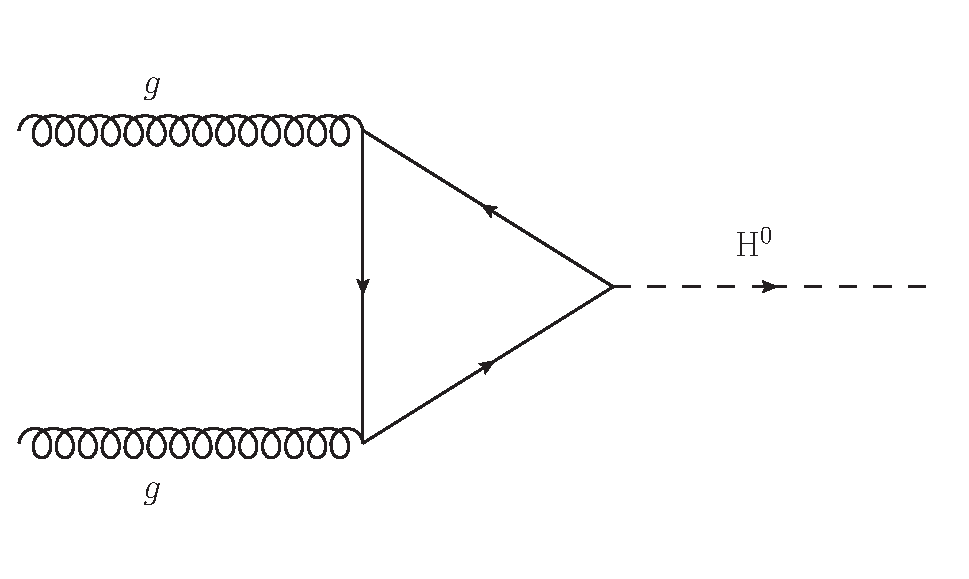
\includegraphics[width=0.4\textwidth]{ch2_figs/ggH.pdf}}
    \subfigure[vector boson fusion]{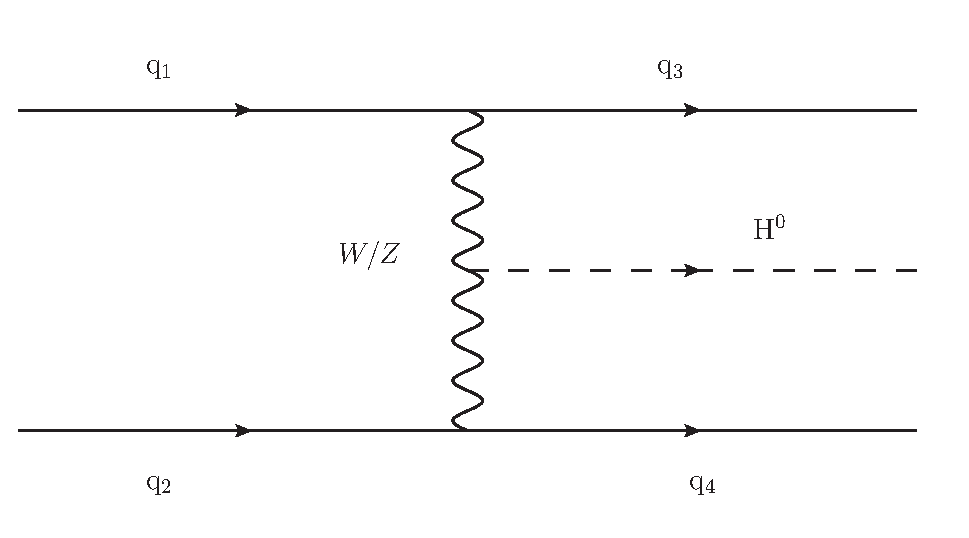
\includegraphics[width=0.4\textwidth]{ch2_figs/VBFH.pdf}}
    \subfigure[Higgs-strahlung]{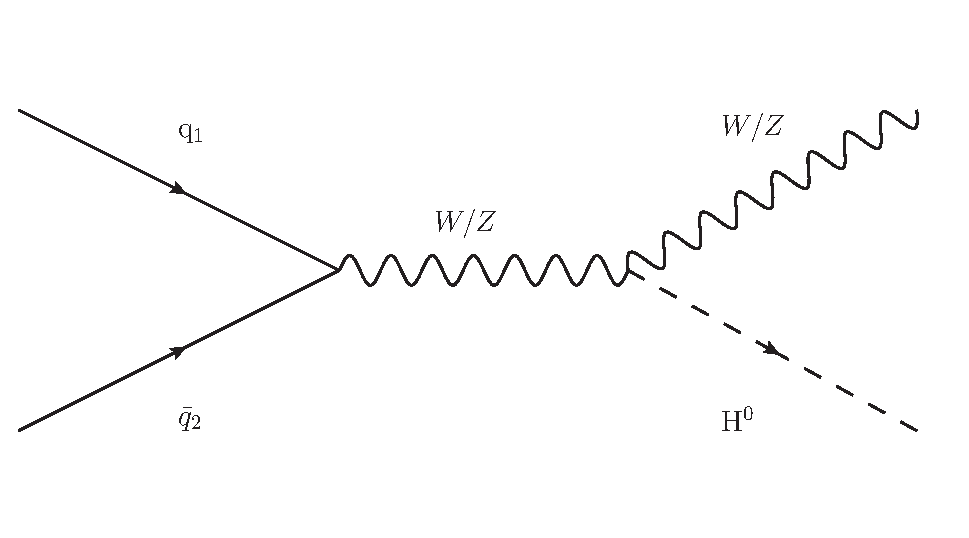
\includegraphics[width=0.4\textwidth]{ch2_figs/VH.pdf}}
    \subfigure[associated production]{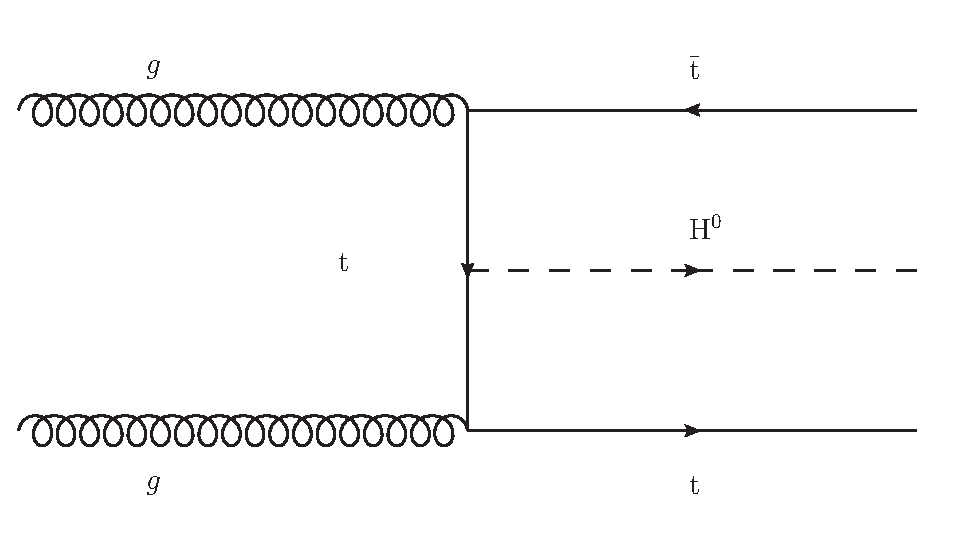
\includegraphics[width=0.4\textwidth]{ch2_figs/ttH.pdf}}
    \caption[Higgs boson production modes at the LHC]{Higgs boson production modes at the LHC:
      gluon fusion $gg\to{}H$ (a), vector boson fusion $qq\to{}qqH$ (b),
      Higgs-strahlung $q\bar{q}\to{}W(Z)H$ (c), and associated
      production $gg\to{}t\bar{t}H$ (d).}
    \label{fig:higgs_production}}
\end{figure}

\begin{figure}[hbtp]
 \begin{center}
   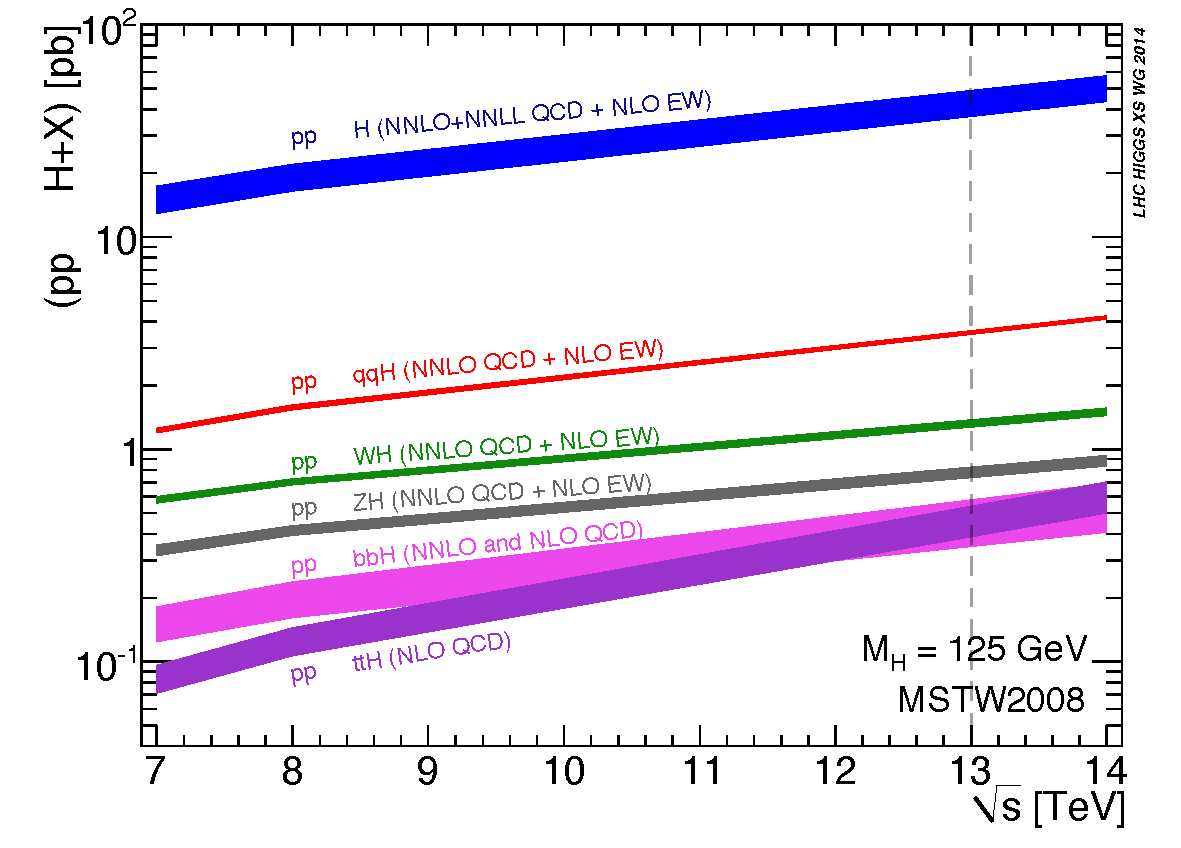
\includegraphics[width=0.8\textwidth]{ch2_figs/higgs_prod_xsec.pdf}
   \caption{Higgs production process cross section as a function of center-of-mass LHC collision energy~\cite{lhchxswg}.
     This dissertation analyzes events produced at 13 TeV.}
   \label{fig:higgs_prod_plot}
 \end{center}
\end{figure}


The decay modes of the Higgs are important in the context of an experimental collider search. The Higgs decay mode and to some extent, the production mode
determine which decay channels are most relevant for an experimental search. After being produced, the Higgs decays almost instantly\footnote{
The Higgs has lifetime of $10^{-22}s$~\cite{pdg}} to pairs of identical SM particles. The probability of the Higgs decaying into a pair of SM particles,
more commony referred to as the branching fraction, depends
on the type of final state particles. The Higgs couples more strongly to massive particles and less strongly to lighter particles. This means a decay to heavy
particles is more likely than a decay to light particles. This is true with the caveat that this effect is balanced by the fact that the Higgs itself has a
finite mass of approximately 125 GeV, and decaying to a particle pair with mass greater than the Higgs mass is strongly suppressed. Decays to heavier
states, such as $H\rightarrow WW$ are allowed, but at least one W is produced with a lighter mass, called an off-shell particle. It is the decay to off-shell
particles that supresses the branching fraction. The greater the off-shell particle's mass differs from the pole mass, the larger the supression.
This explains some of the decay mode behavior as a function of Higgs mass in
Figure~\ref{fig:higgs_decay}.

\begin{figure}[hbtp]
 \begin{center}
   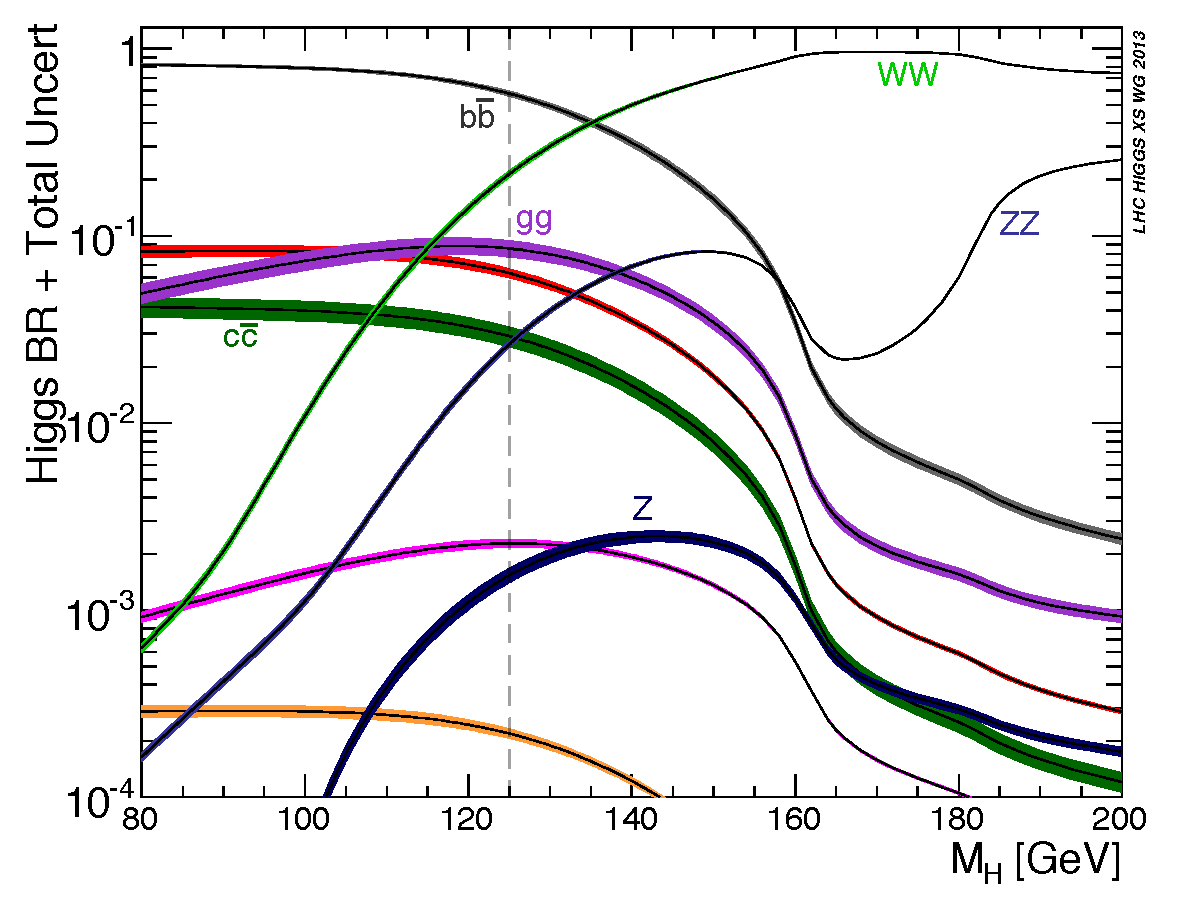
\includegraphics[width=0.8\textwidth]{ch2_figs/higgs_decay.pdf}
   \caption{Higgs branching fractions as a function of Higgs mass~\cite{lhchxswg}.}
   \label{fig:higgs_decay}
 \end{center}
\end{figure}

While the Higgs discovery represents significant progress in verifying the predictions of the SM, many important questions remain. Do the observed properties
of the Higgs exactly match the SM expectations? Do particle masses, specifically the top quark, come from their coupling to the Higgs or is there another
explanation? A thorough study and understanding of \tth processes can address these questions.  

\section{ttH}
\subsection{Description}
In a broader theoretical context, \tth searches are in essence a probe of the SM, \emph{directly} testing the Yukawa coupling strength of the Higgs boson to top quarks. The fact that a
measurement of \tth is a direct probe is an important distinction between an indirect probe. As mentioned previously, the Higgs was discovered and proven
consistent with the SM via the gluon fusion production mode in Figure~\ref{fig:higgs_production}. The gluon fusion diagram includes a fermion loop (triangle)
that produces the Higgs. Because the Higgs couples more strongly to massive particles, the fermion that runs around this loop is assumed to be, and consistent
with the massive top quark. And
because the Higgs was already confirmed and consistent with SM predictions after being produced this way, the top-Higgs Yukawa coupling has already been
measured, albeit \emph{indirectly}. Beacuse we don't have direct evidence that the fermion running around the gluon fusion loop is the top quark, further
confirmation of the top-Higgs Yukawa coupling is necessary. Enter \tth. While the primary goal of searching for \tth has been motivated,
other important questions about the SM can be addressed simultaneously. The top quark is unique with respect to all other quarks. It is the heaviest, but curiously
its relative mass difference with respect to the next heaviest quark is more than 4x greater than any other relative quark mass difference. The top quark mass
being so much greater than any other quark inspires questions about the pattern of the quark masses. Does the top quark's mass come only from the Higgs? Or could
it also come from something beyond the SM? Direct \tth searches will help answer these questions. 

%% \begin{figure}[hbtp]
%%  \begin{center}
%%    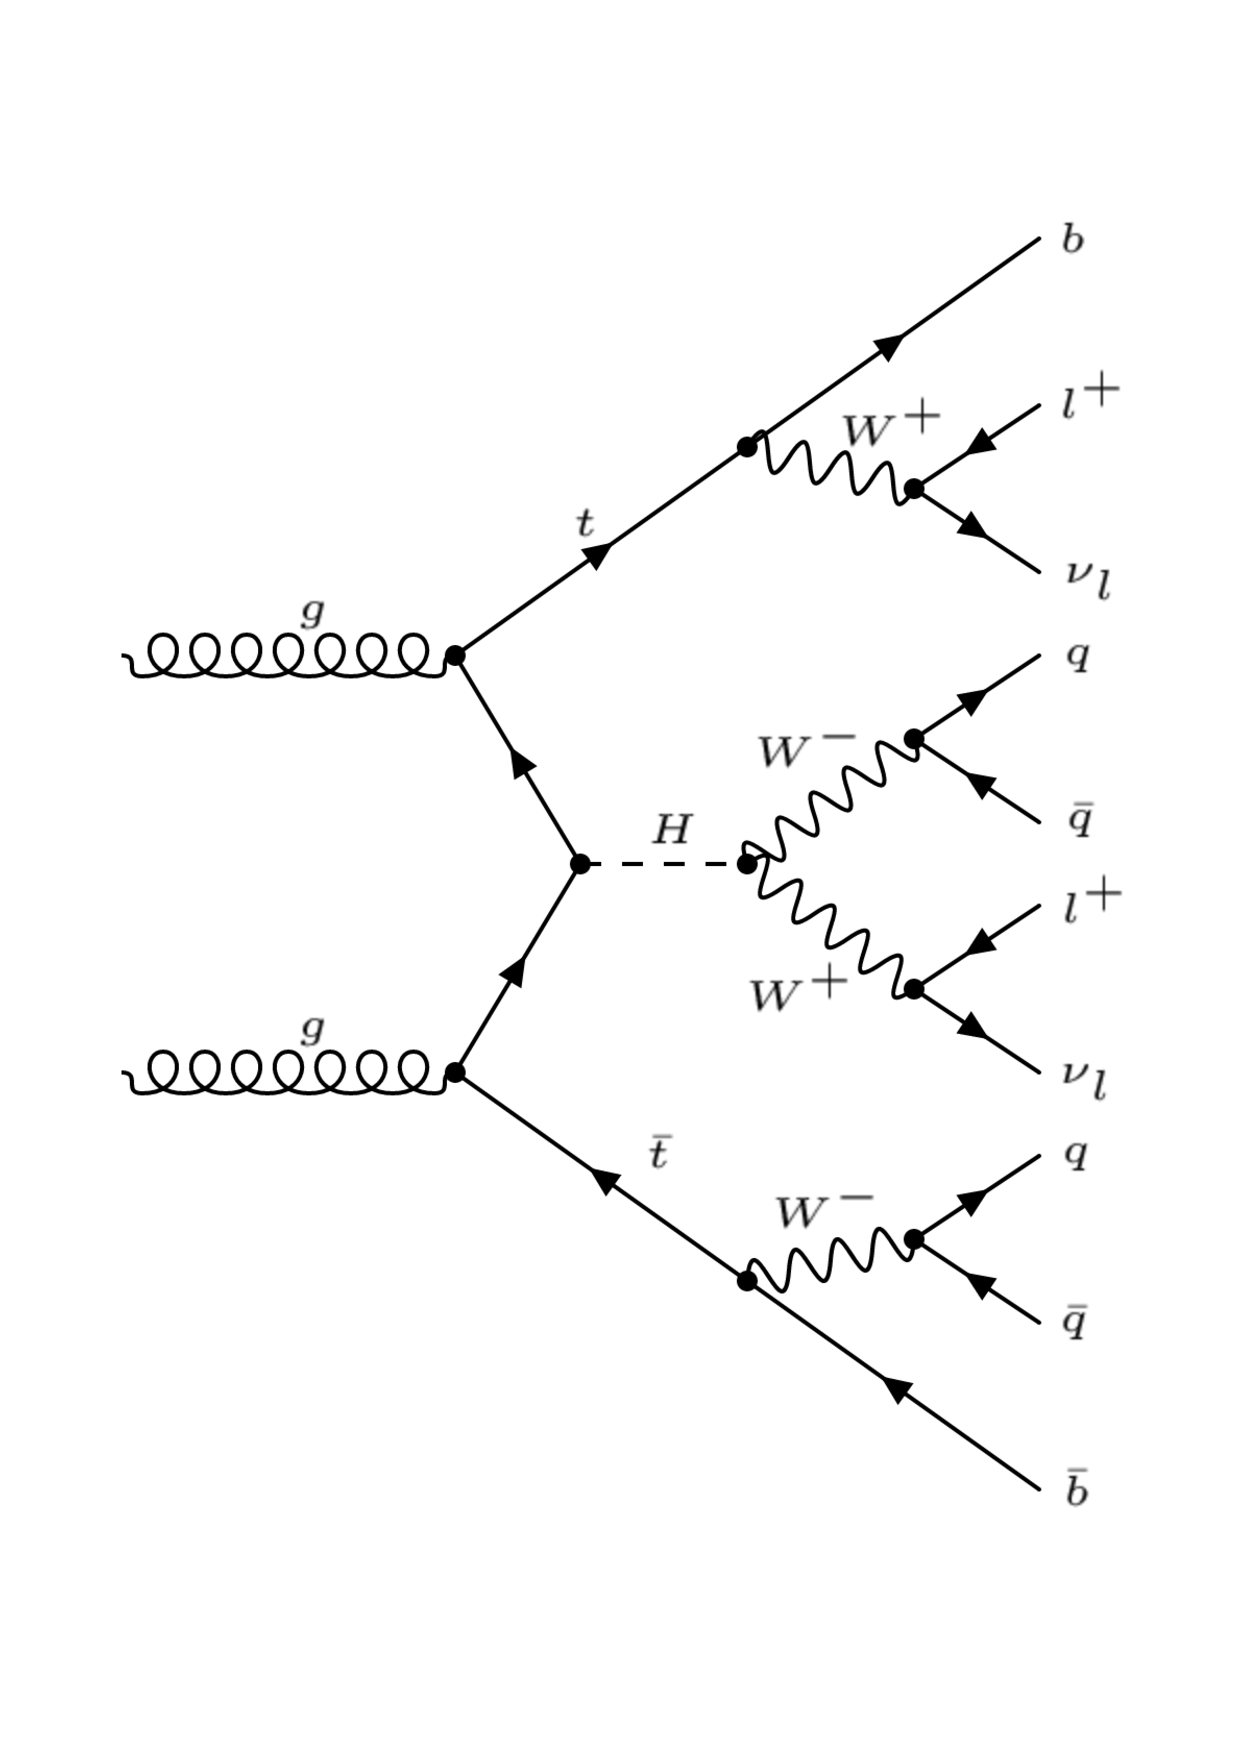
\includegraphics[width=0.4\textwidth]{ch2_figs/feynman_diagram_ttH_HWW_2lss.pdf}
%%    \caption{A \tth process at the LHC. The final state here is one of the targets of the analysis presented later in this dissertation.}
%%    \label{fig:tth_example_diagram}
%%  \end{center}
%% \end{figure}

In an experimental context, the \tth process, or more commonly referred to as simply \tth, is produced by two gluons, each decaying to a top-antitop quark pair, where a top and an
antitop from each gluon combine to form a Higgs boson, represented by the feynman diagram in Figure~\ref{fig:tth_example_diagram}.
The remaining top and antitop quark decay to a W boson and b quark with nearly 100$\%$ probability
\footnote{While the top can in principle decay to quark flavors other than bottoms, these decays are so heavily CKM suppressed\cite{CKM} that they are
neglected.}. The W boson produced in the top decays instantly to pairs of SM particles. These pairs include a charged lepton and a neutrino of the same
flavor approximately 1/3 of the time, while the rest of the time~\cite{pdg} the W decays to a quark-antiquark where the quark and antiquark have different flavors. 
Like the W, the Higgs is free to decay to numerous states according to Figure~\ref{fig:higgs_decay}. Because of the various decay modes of the Higgs and
the Ws there are many final states possible in \tth. These numerous possible final states dictate the experimental techniques employed in searches,
with completely separate analysis efforts dedicated to a single \tth higgs final state, or a closely related collection of Higgs final states.


\subsection{Multilepton Final States}
The specific signal targeted by this analysis is \tth decaying to final states with two or more charged leptons. Examples of this signal are in
Figure~\ref{fig:tth_example_diagram}. There are multiple Higgs decays included this definition, specificaly WW, ZZ and $\tau\tau$. The fractions of these Higgs decays
is in Figure~\ref{fig:pie}. 

\begin{figure}[htb]
\centering
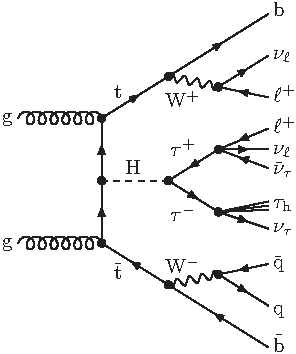
\includegraphics[width=0.25\linewidth]{ch2_figs/gg-ttH-tt-2lss.pdf}
\hspace{0.5cm}
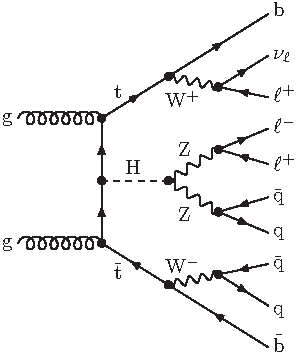
\includegraphics[width=0.25\linewidth]{ch2_figs/gg-ttH-ZZ-3l.pdf}
\hspace{0.5cm}
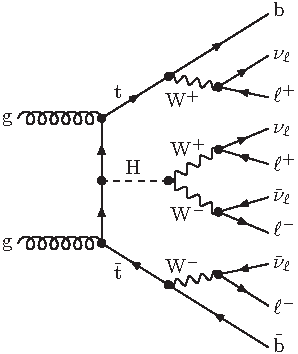
\includegraphics[width=0.25\linewidth]{ch2_figs/gg-ttH-WW-4l.pdf}
\caption{Examples of leading order Feynman diagrams for $t\bar{t}H$ production at pp colliders, with the Higgs boson decaying to
$\tau\tau$, $\mathrm{ZZ}^{*}$, and
$\mathrm{WW}^{*}$ (from left to right). The first, second, and third diagrams are examples of the two same-sign lepton signature,
the three lepton signature, and the four lepton signature, respectively.}
\label{fig:tth_example_diagram}
\end{figure}

\begin{figure}[hbtp]
 \begin{center}
   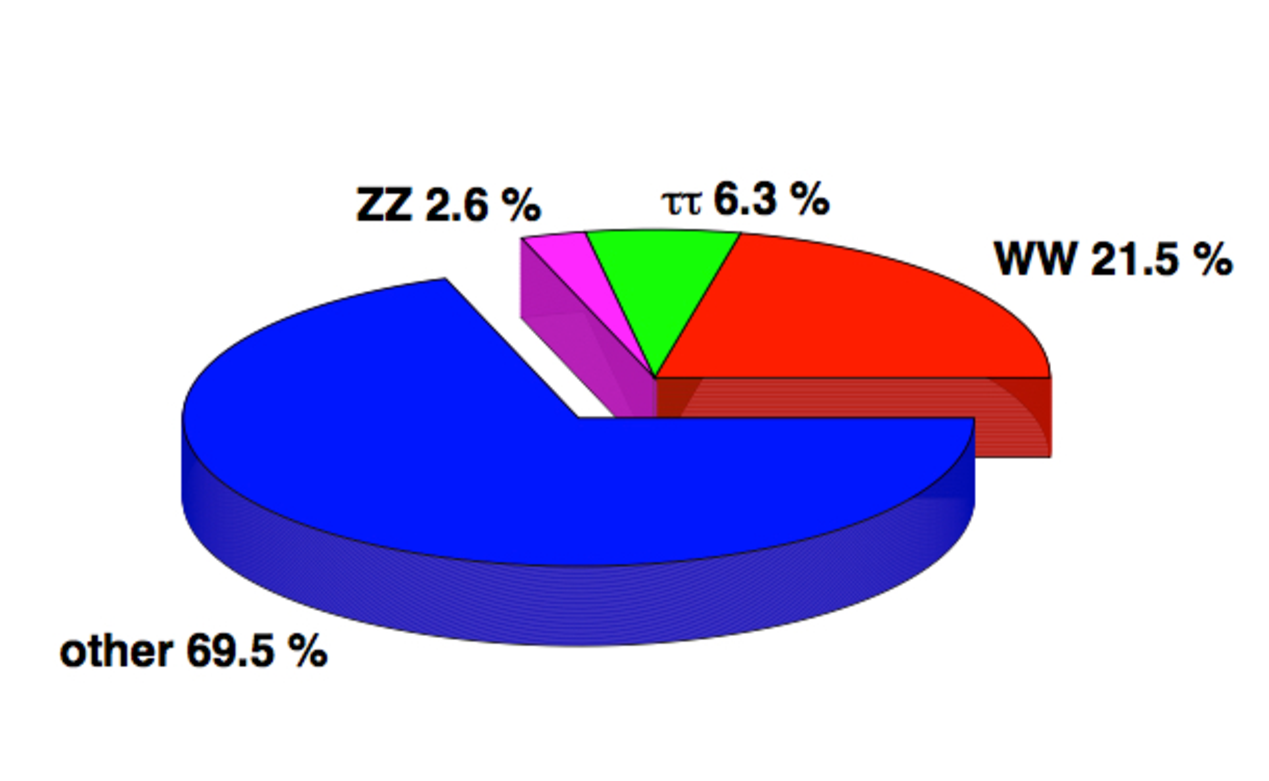
\includegraphics[width=0.4\textwidth]{ch2_figs/pie.pdf}
   \caption{The Higgs branching fractions assuming a mass of 125 GeV. The slices removed are the decays targeted in this analysis.}
   \label{fig:pie}
 \end{center}
\end{figure}

% % uncomment the following lines,
% if using chapter-wise bibliography
%
% \bibliographystyle{ndnatbib}
% \bibliography{example}
